\item {\color{red} (50 pts)} \textbf{Backtracking line search}. Please show the convergence of backtracking line search on a $m$-strongly convex and $M$-smooth objective function $f$ as
$$
f\left(\mathbf{x}^{(k)}\right)-p^{\star} \leq c^k\left(f\left(\mathbf{x}^{(0)}\right)-p^{\star}\right)
$$
where $c=1-\min \{2 m \alpha, 2 \beta \alpha m / M\}<1$.

\begin{figure}[htbp]
    \centering
	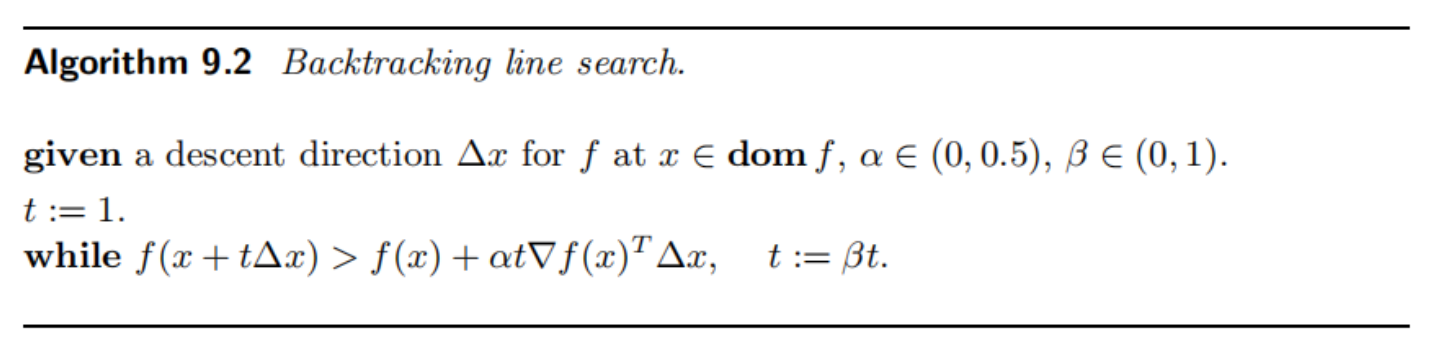
\includegraphics[width=1\textwidth]{./image/backtracking.png}
\end{figure}

\solution{}
Since $f$ is convex and $M$-smooth, so we could expand $f(\mathbf{x}+t\Delta \mathbf{x})$ at $\mathbf{x}$:
\begin{align*}
    f(\mathbf{x}+t\Delta \mathbf{x}) &\leq f(\mathbf{x})+\nabla f(\mathbf{x})^T(t\Delta\mathbf{x}) +\dfrac{M}{2}\|t\Delta \mathbf{x}\|^2\\
    &= f(\mathbf{x})+t\nabla f(\mathbf{x})^T\Delta \mathbf{x}+\dfrac{M}{2}t^2\|\Delta \mathbf{x}\|^2
\end{align*}
Since the backtracking line search would terminate when
$$f(\mathbf{x}+t\Delta \mathbf{x})\leq f(\mathbf{x})+\alpha t\nabla f(\mathbf{x})^T\Delta \mathbf{x}$$
If we let the $f(\mathbf{x}+t\Delta \mathbf{x})$'s upper bound 
$f(\mathbf{x})+t\nabla f(\mathbf{x})^T\Delta \mathbf{x}+\dfrac{M}{2}t^2\|\Delta \mathbf{x}\|^2$ to be less than\\
$f(\mathbf{x})+\alpha t\nabla f(\mathbf{x})^T\Delta \mathbf{x}$, then it must have been terminated.\\
So we have:
\begin{align*}
    f(\mathbf{x})+t\nabla f(\mathbf{x})^T\Delta \mathbf{x}+\dfrac{M}{2}t^2\|\Delta \mathbf{x}\|^2 &\leq f(\mathbf{x})+\alpha t\nabla f(\mathbf{x})^T\Delta \mathbf{x} \\
    \dfrac{M}{2}t^2\|\Delta \mathbf{x}\|^2 &\leq (\alpha-1) t\nabla f(\mathbf{x})^T\Delta \mathbf{x} \\
    \dfrac{M}{2}t\|\Delta \mathbf{x}\|^2 &\leq (\alpha-1)\nabla f(\mathbf{x})^T\Delta \mathbf{x} \text{\ \ \ \ \ \ \ \ \ \ \ \ (Since $t>0$)}\\
    t &\leq \dfrac{2(\alpha-1)\nabla f(\mathbf{x})^T\Delta \mathbf{x}}{M\|\Delta \mathbf{x}\|^2}
\end{align*}

Since $\alpha\in(0,0.5)$, so $(\alpha-1)<0$, and since $\Delta \mathbf{x}$ is the descent direction, so $\nabla f(\mathbf{x})^T\Delta \mathbf{x}<0$, so $t$ is less than a positive number.\\
Since $t$ is generated by the backtracking line search, so we have $t\leq \dfrac{\beta\cdot 2(\alpha-1)\nabla f(\mathbf{x})^T\Delta \mathbf{x}}{M\|\Delta \mathbf{x}\|^2}$.
Also, the initial step is $t=1$, so combine the above inequality, we have:
$$t=\min\left\{1,\dfrac{\beta\cdot 2(\alpha-1)\nabla f(\mathbf{x})^T\Delta \mathbf{x}}{M\|\Delta \mathbf{x}\|^2}\right\}$$

\textbf{And for this problem, we take the descent direction as $\Delta \mathbf{x}=-\nabla f(\mathbf{x})$, so we have:}
$$t=\min\left\{1,\dfrac{\beta\cdot 2(\alpha-1)\nabla f(\mathbf{x})^T(-\nabla f(\mathbf{x}))}{M\|-\nabla f(\mathbf{x})\|^2}\right\}=\min\left\{1,\dfrac{2\beta(1-\alpha)}{M}\right\}$$

Since $\mathbf{x}^{(k+1)}=\mathbf{x}^{(k)}+t\Delta\mathbf{x}$, we have 
\begin{align*}
    f\left(\mathbf{x}^{(k+1)}\right) &= f\left(\mathbf{x}^{(k)}+t\Delta\mathbf{x}^{(k)}\right) \\
    &= f\left(\mathbf{x}^{(k)}-t\nabla f\left(\mathbf{x^{(k)}}\right)\right) \\
    &\leq f\left(\mathbf{x}^{(k)}\right)+\alpha t\nabla f\left(\mathbf{x}^{(k)}\right)^T\Delta \mathbf{x}^{(k)} \\
    &= f\left(\mathbf{x}^{(k)}\right)\alpha t\left\|\nabla f\left(\mathbf{x}^{(k)}\right)\right\|^2 \\
    &= f\left(\mathbf{x}^{(k)}\right) - \alpha\cdot\min\left\{1,\dfrac{2\beta(1-\alpha)}{M}\right\} \left\|\nabla f\left(\mathbf{x^{(k)}}\right)\right\|^2
\end{align*}

To continously prove, we need to introduce the Lemma:
$f(\mathbf{x})$ is $m$-strongly convex, then $$p^*\geq f(\mathbf{x})-\dfrac{1}{2m}\|\nabla f(\mathbf(x))\|^2$$
proof:
Since $f$ is $m$-strongly convex, so we have $\forall \mathbf{x}, \mathbf{y}$:
$$f(\mathbf{y})\geq f(\mathbf{x})+\nabla f(\mathbf{x})^T(\mathbf{y}-\mathbf{x})+\dfrac{m}{2}\|\mathbf{y}-\mathbf{x}\|^2$$
Let $$g(\mathbf{y})= f(\mathbf{x})+\nabla f(\mathbf{x})^T(\mathbf{y}-\mathbf{x})+\dfrac{m}{2}\|\mathbf{y}-\mathbf{x}\|^2$$
So $\nabla g(\mathbf{y})=\nabla f(\mathbf{x}) + m(\mathbf{y}-\mathbf{x})$, and $\nabla^2g(\mathbf{y})=mI\succeq 0$, so 
$$g(\mathbf{y})_{\min}=g\left(\mathbf{x}-\dfrac{1}{m}\nabla f(\mathbf{x})\right)=f(\mathbf{x})-\dfrac{1}{2m}\|\nabla f(\mathbf{x})\|^2$$
So 
$$f(\mathbf{y})\geq f(\mathbf{x})-\dfrac{1}{2m}\|\nabla f(\mathbf{x})\|^2$$
Change $\mathbf{y}$ to $p^*$, we have $p^*\geq f(\mathbf{x})-\dfrac{1}{2m}\|\nabla f(\mathbf{x})\|^2$.\\
So we have proved the Lemma.\\
So we get that
$$\|\nabla f(\mathbf{x})\|^2\geq (2m)\left(f(\mathbf{x})-p^*\right)$$

With the Lemma, we can get that
\begin{align*}
    f\left(\mathbf{x}^{(k+1)}\right) &\leq f\left(\mathbf{x}^{(k)}\right) - \alpha\cdot\min\left\{1,\dfrac{2\beta(1-\alpha)}{M}\right\}\left\|\nabla f\left(\mathbf{x^{(k)}}\right)\right\|^2\\
    f\left(\mathbf{x}^{(k+1)}\right)-p^* &\leq f\left(\mathbf{x}^{(k)}\right) - p^* - \alpha\cdot\min\left\{1,\dfrac{2\beta(1-\alpha)}{M}\right\}\left\|\nabla f\left(\mathbf{x^{(k)}}\right)\right\|^2\\
    f\left(\mathbf{x}^{(k+1)}\right)-p^* &\leq f\left(\mathbf{x}^{(k)}\right) - p^* - \alpha\cdot\min\left\{1,\dfrac{2\beta(1-\alpha)}{M}\right\}(2m)\left(f\left(\mathbf{x^{(k)}}\right)-p^*\right) \text{\ \ \ \ \ \ (Lemma)} \\
\end{align*}


% \mathbf{x}






